%======================================================================
\section{User acceptance test --- Sunday 25 October 2026}\label{sec:uat}
%======================================================================

\textbf{What was tested.} Keystone.app (\eref{FND-02}), built from \code{bw/fnd06-mod01-patterns}, used by you on
real files: the Vector vault and the Leonardo gearbox. Your list is in the Apple Note ``FreeCAD UAT'' (eight
screenshots), and more requests came in during the day. Every fix below is a \code{[BW]} commit (not pushed),
was tested on a throwaway profile against a \emph{copy} of the files (the real vault was only read), and
is in the Keystone build now in \file{/Applications} (\code{1.1.4-bw.1+4d1d982}).

\subsection{Your list}
\begin{center}
\small
\begin{longtable}{@{}p{0.5cm}p{5.0cm}p{1.6cm}p{8.2cm}@{}}
\toprule
\# & You saw & Status & What changed\\
\midrule\endhead
\bottomrule\endfoot
1 & Warnings when the vault sidebar opened & Fixed & FreeCAD~1.1's first-start page overwrote the Vector Labs
  theme with a stock one that lacks the panel tokens. The first-start page no longer runs, and a profile it
  already overwrote is healed. The 16 panel tokens were also added to FreeCAD Light/Dark
  (\code{a5bedb6}, \eref{UIX-01}).\\
2 & Ribbon buttons not all visible & Fixed & Two causes. Mostly \#10 below (whole groups empty). And in a
  narrower window Qt gave the first groups their full width and squeezed the last ones to one button and
  \guillemotright, cutting their captions (``CON\ldots T''). The tools row is now shared out: the groups shrink
  together, none below its caption's width; the rest of a group is under \guillemotright{} and its caption
  menu. Checked at 2056, 1512 and 1028\,px wide (\code{b59bf0a}, \eref{UIX-06}).\\
3 & Vault sidebar transparent & Fixed & The floating vault card is gone: its list is the Start page's
  \emph{Files} tab (\code{1c3389e}, \eref{PDM-10}).\\
4 & All drawings as a drawing tree, other views for assembly trees & Fixed & Files is one indented tree:
  each top assembly with its parts and their drawings under them (\S\ref{sec:uat-files};
  \code{0087827}).\\
5 & ``The vault sidebar needs to be something else'' & Fixed & As \#3: the vault is browsed on the Start
  page only (your choice).\\
6 & Better rendering, with textures & Fixed & Your choice, the Fusion-like studio: soft lights and studio
  reflections, each part coloured and finished from its material (brushed aluminium, steel, ABS, PETG), a hand
  colour kept; off in Preferences $>$ BruceWorx (stock FreeCAD). No cost in speed on the gearbox
  (\code{5cbf03e}, \S\ref{sec:uix08-plan}, \eref{UIX-08}).\\
7 & Odd font (halo) in the sidebar & Fixed & The transparent Browser draws a halo behind its text in
  the card colour, a theme token. Your profile was in FreeCAD Light then (\#1), which lacked the token, so
  Qt kept the overlay's built-in 30\,\% black: a dark smudge round every row. The halo now always contrasts
  with the text (light behind dark text, dark behind light), whatever the theme (\code{f3b6c7e},
  \eref{UIX-03}).\\
8 & Section view crashes & Fixed & Coin~4.0.3 crashed tearing down a dragged dragger; Coin~4.0.10 now, and the
  handles' callbacks go through the view, which holds the GIL (\code{d519d29}). Later the same day: the
  Section button is a toggle and faces are found (\S\ref{sec:uat-section}).\\
9 & Trackpad: two fingers pan, Shift zoom, Cmd orbit & Fixed & The Vector Labs swipe handling
  (Shift panned, a plain swipe zoomed) is swapped: a plain swipe pans with the fingers, Shift + swipe zooms at
  the pointer, Cmd + swipe orbits about the point a mouse orbit picks. A mouse wheel and pinch are unchanged,
  in every navigation style; Revit stays. Off switch on Preferences $\rightarrow$ BruceWorx
  (\code{4eed4ca}, \eref{UIX-13}). Tested with synthetic swipes; to try on the real trackpad.\\
10 & Sketch/Modeling buttons gone after switching tabs & Fixed & Reproduced with a copy of your settings:
  the first time a tab showed, all its groups but the last had captions and no buttons. The macOS title row
  makes the window's content reach under the title strip, and Qt gives a widget there a 40\,px top
  margin. A tab's groups wait hidden at the top left, so they got it; shown in their row they lost it, but
  their layout kept buttons 0\,px tall. Toolbars now ignore the title strip, as the docks already did
  (\code{c4a644a}, \eref{UIX-06}).\\
\end{longtable}
\end{center}

\subsection{Files: one tree, pictures on hover, where used}\label{sec:uat-files}
Your requests: ``make the files look like a drawing tree with indents; pictures should be tooltips'', then
``combine the file and structure trees'' with where-used. There is one tab (Figure~\ref{fig:uat-files}):
\begin{itemize}
  \item \textbf{Tree.} Each top assembly, its parts and sub-assemblies indented with quantities, every item's
        drawings directly under it, then \emph{Not in an assembly}. One line per file: P/N-REV, description,
        qty, state, status (and \emph{Get latest}). Sorted by part number, like a BOM; the sort button swaps
        to Modified. An assembly checked in without a recorded BOM gets its lines from the links in its file
        (\file{bruceworx/vault\_trees.py}).
  \item \textbf{Where used.} Selecting a file tints the assemblies above it and its other rows elsewhere in
        the tree; the footer names the assemblies that use it, e.g.\ ``used in 1 assembly:
        LE-02-01002-001-01 $\times$3''. An assembly's own parts are not tinted: the tree already lists them
        under it.
  \item \textbf{Search and chips} keep the matches' parents, dimmed. Folded branches stay folded.
  \item \textbf{Pictures} moved to the file name's tooltip.
\end{itemize}
The \emph{Structure} tab built in the morning was folded into this tree. It also had the ``parts without a
drawing'' list, which can come back as a filter chip if you want it.

\begin{figure}[h]
  \centering
  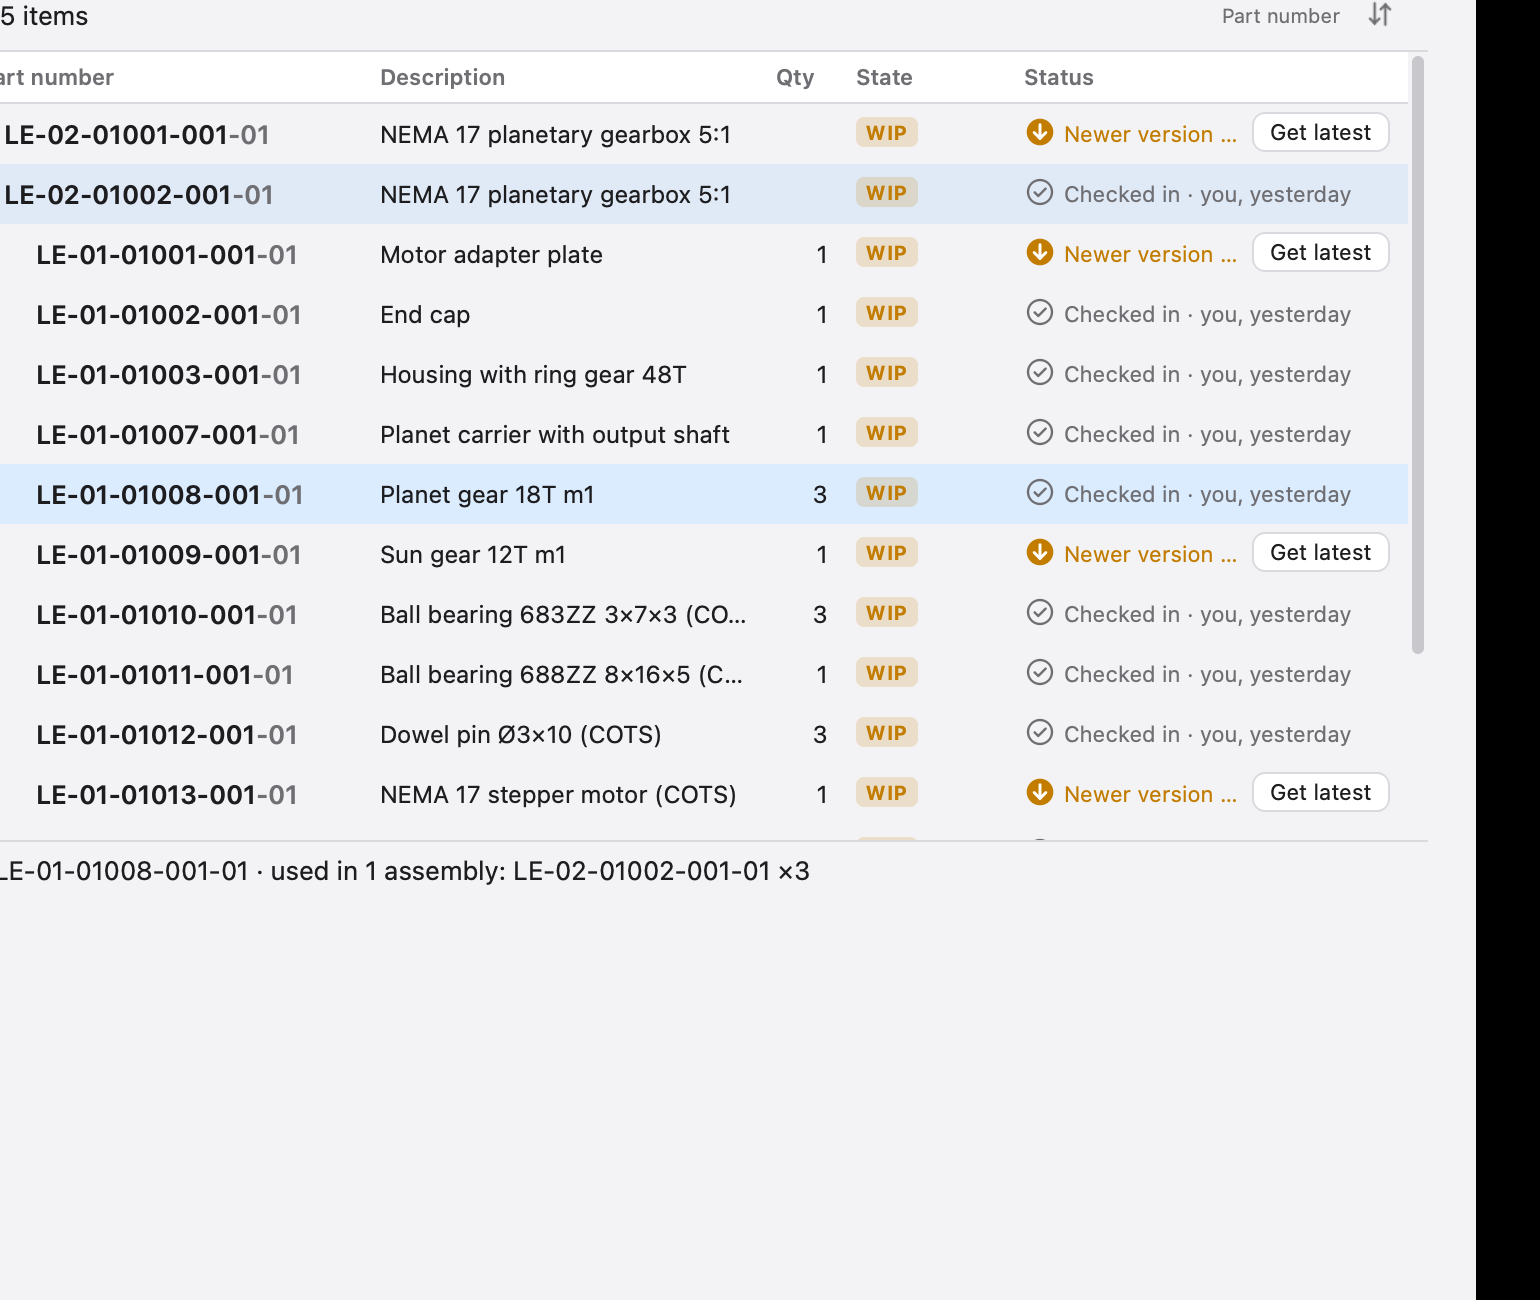
\includegraphics[width=0.78\linewidth]{fig/uat_files_tree.png}
  \caption{The Files tab on Vector: the gearbox's twelve parts under it, the planet gear selected; its
    assembly is tinted and the footer says where it is used.}\label{fig:uat-files}
\end{figure}

\subsection{Iso pictures}
Your request: ``the renders in the file list should be an iso view of the model where the part or assembly is
centred''. The picture is drawn off screen in the isometric view, fitted and centred; the views on screen do
not move, and joints, origins, datums and sketches are left out (\file{bruceworx\_preview.py},
\code{225d2fb}). Your choices: only \emph{check-ins} write it into the file (ordinary saves keep FreeCAD's
snapshot), and only when the file is becoming a new version anyway; files checked in before are drawn once by
\emph{Refresh Pictures} in the Files menu into a cache on this Mac, never into the vault.
On the Vector copy: 14 pictures in 3.6\,s, none left open (LE-02-01001 has nothing to draw). One gap: an
assembly whose work copies are older than the vault is drawn from the stored file, where its parts may not be
found.

\begin{figure}[h]
  \centering
  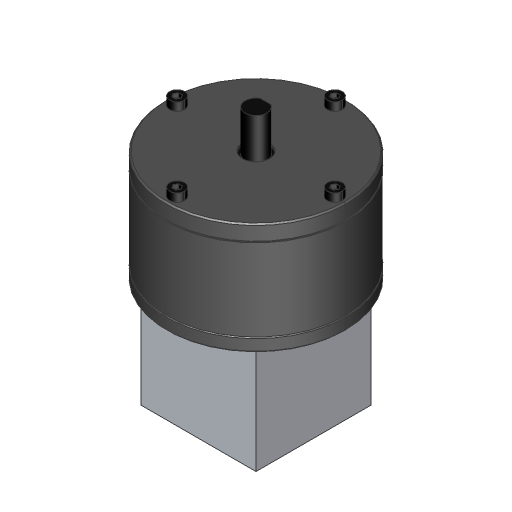
\includegraphics[width=0.3\linewidth]{fig/uat_iso_assembly.png}\hspace{2em}
  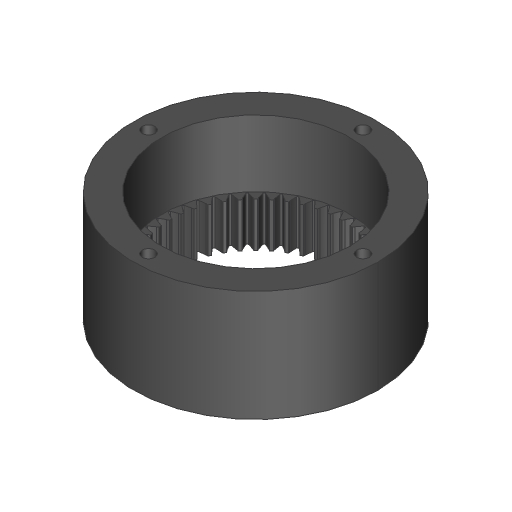
\includegraphics[width=0.3\linewidth]{fig/uat_iso_checkin.png}
  \caption{Left: the gearbox from Refresh Pictures. Right: the housing's thumbnail after a check-in made with
    the view turned to Top.}
\end{figure}

\subsection{Section view: on and off, on a face}\label{sec:uat-section}
Your report: ``I tried it once and then shut it off; now it won't work. I should be able to select a face and
make a section from that face.'' Three causes (\code{b50e8b5}, \eref{MOD-16}):
\begin{itemize}
  \item \textbf{No off switch.} The nav pill's Section button only ever made another section; the only off was
        View $\rightarrow$ Sections Off. The button is now a toggle: down while a section is on, pressed again
        turns sections off; pressed with nothing selected it brings the last section back; with a face selected
        it cuts on that face. It works while its own Section tab is open (the tab's edits are kept) and is
        greyed while another tool edits.
  \item \textbf{Faces were ignored.} A face picked inside a body or an assembly comes as a path
        (\code{Housing.Body.Hole.;\#74:1;:Hf06,F.Face1}); only a bare \code{Face1} was recognised, so every
        section fell back to XZ.
  \item \textbf{Fit All fitted the ground grid} (2\,m across): the model was a speck, picks landed on the grid.
        The grid is now left out of the bounding box (\eref{FND-08}).
\end{itemize}

\subsection{Joint markers}
Your request: ``the joints are way too intense; more wireframe and much smaller''. Joint coordinate systems are
drawn at about half the size with thin axes, the grey filled disc now an outline; the grounded padlock is half
the size and an outline (Figure~\ref{fig:uat-joints}; \code{4d1d982}, \eref{ASM-03}). Not yet tried by hand:
whether the thinner lines are still easy to click.

\begin{figure}[h]
  \centering
  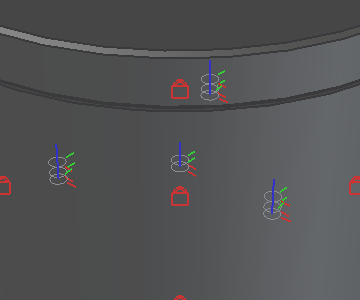
\includegraphics[width=0.36\linewidth]{fig/uat_joint_markers.png}
  \caption{Gearbox joints after the change: outline discs, thin axes, small outline padlocks.}\label{fig:uat-joints}
\end{figure}

\subsection{Still open}
Nothing from this list. Closed later the same day: MOD-14 on-canvas editing is on (the teardown fix went in with it,
\code{e79f38a}), and the inspector's acceptance is a GUI test in the repository that passed three runs of three (the
crash was seen only with a scratch script).
